% Set title page for separate titlepage
\documentclass{article}

% Some standard math packages
\usepackage{amsmath}
\usepackage{amssymb}
\usepackage{amsfonts}
\usepackage{pdfpages}
% Package for lists
\usepackage[shortlabels]{enumitem}
% Dashed text
\usepackage{arydshln}
\usepackage[normalem]{ulem}
%rotate page
\usepackage{pdflscape}
% Graphics
\usepackage{tikz}
\usepackage{rotating}
\usepackage{geometry}
\usepackage{pgfgantt}

%Colors
\definecolor{lightblue}{HTML}{4FC3F7}
\definecolor{lightgreen}{HTML}{81C784}
\definecolor{lightorange}{HTML}{FF8A65}

\title{Project monitoring}
%\subtitle{MSc in Computer Science \\ For entry in 2018}

%\author{Luca Dolfi}
\pagestyle{headings}
\markright{Luca Dolfi\hfill \today \hfill}
\begin{document}
%\maketitle
\part*{Project monitoring - version 10}
Each task, at least in the first two milestones, is composed mostly readings and papers review.
At the end of each tasks a small summary will be produced for that task. 
At the end of the milestone all summaries will come together to form a chapter of the final report. \\

\paragraph*{Milestones}
\begin{enumerate}[A)]
\item \sout{Project assessment} COMPLETE 
\item \sout{Concepts of QM} COMPLETE
\item \sout{Concepts of information theory} COMPLETE
\item Investigation into bound information / Final submission
\end{enumerate}

\centerline{
	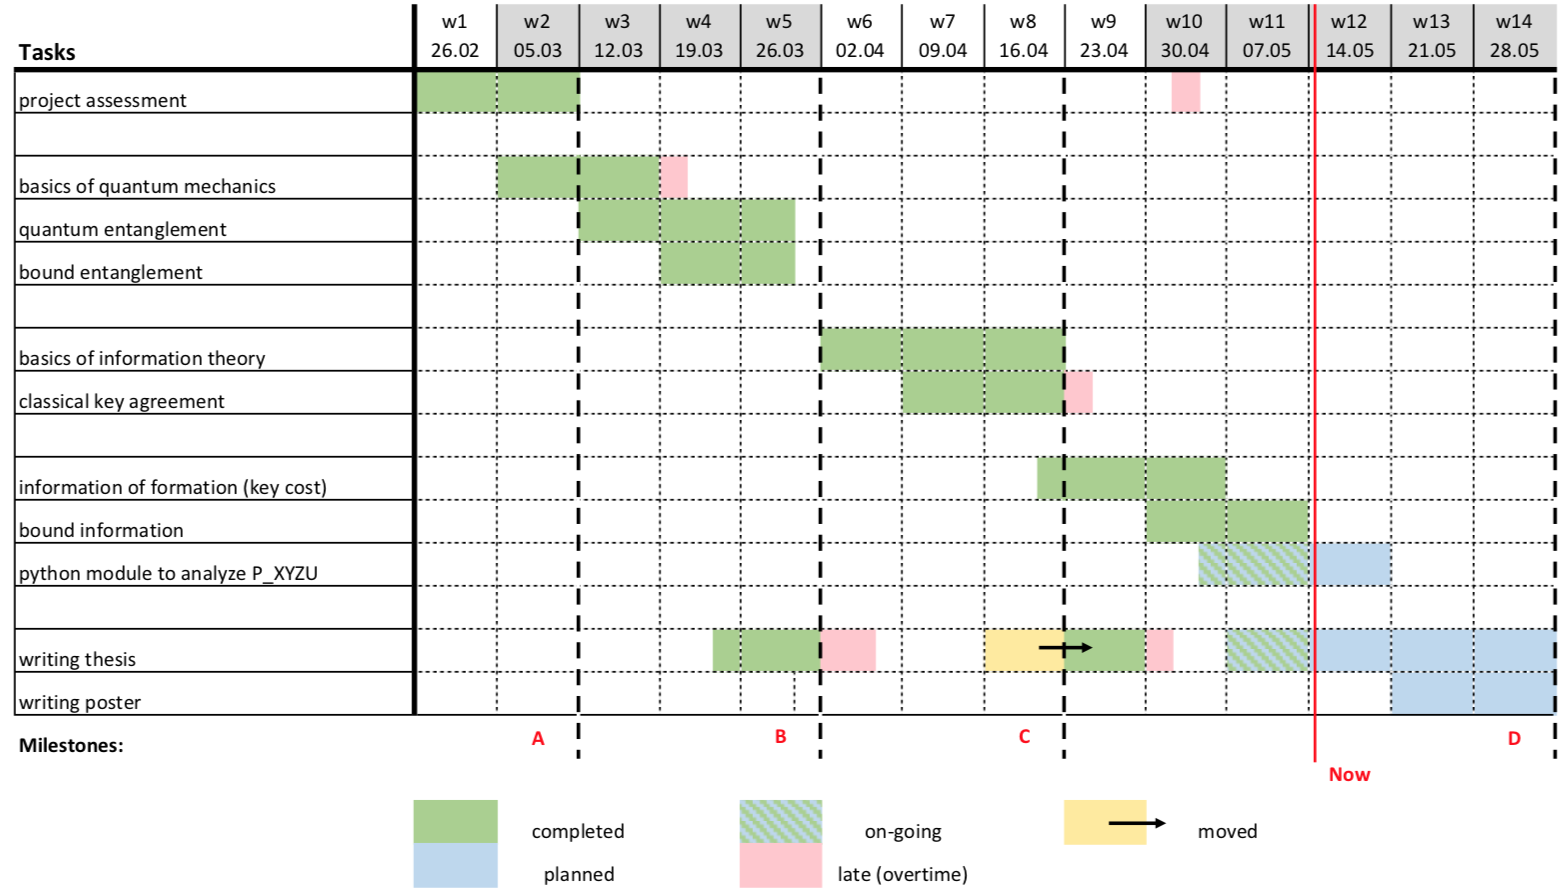
\includegraphics[scale=0.5]{gantt-10.png}
}

\end{document}
